\chapter{Machine Learning based Backtesting}

In the world of machine learning (ML), classification is about sorting things into categories. When applied to trading, ML Models predict whether the price will go up or down based on today's as well as historical data.
Using ML to predict trading outcomes requires a systematic approach.
This structured process is visualized as a pipeline, detailed in fig. \ref{fig:ml_pipeline}.

%trim=left bottom right top,
\section{ML Trading Pipeline}


\begin{figure}[H]
\centering
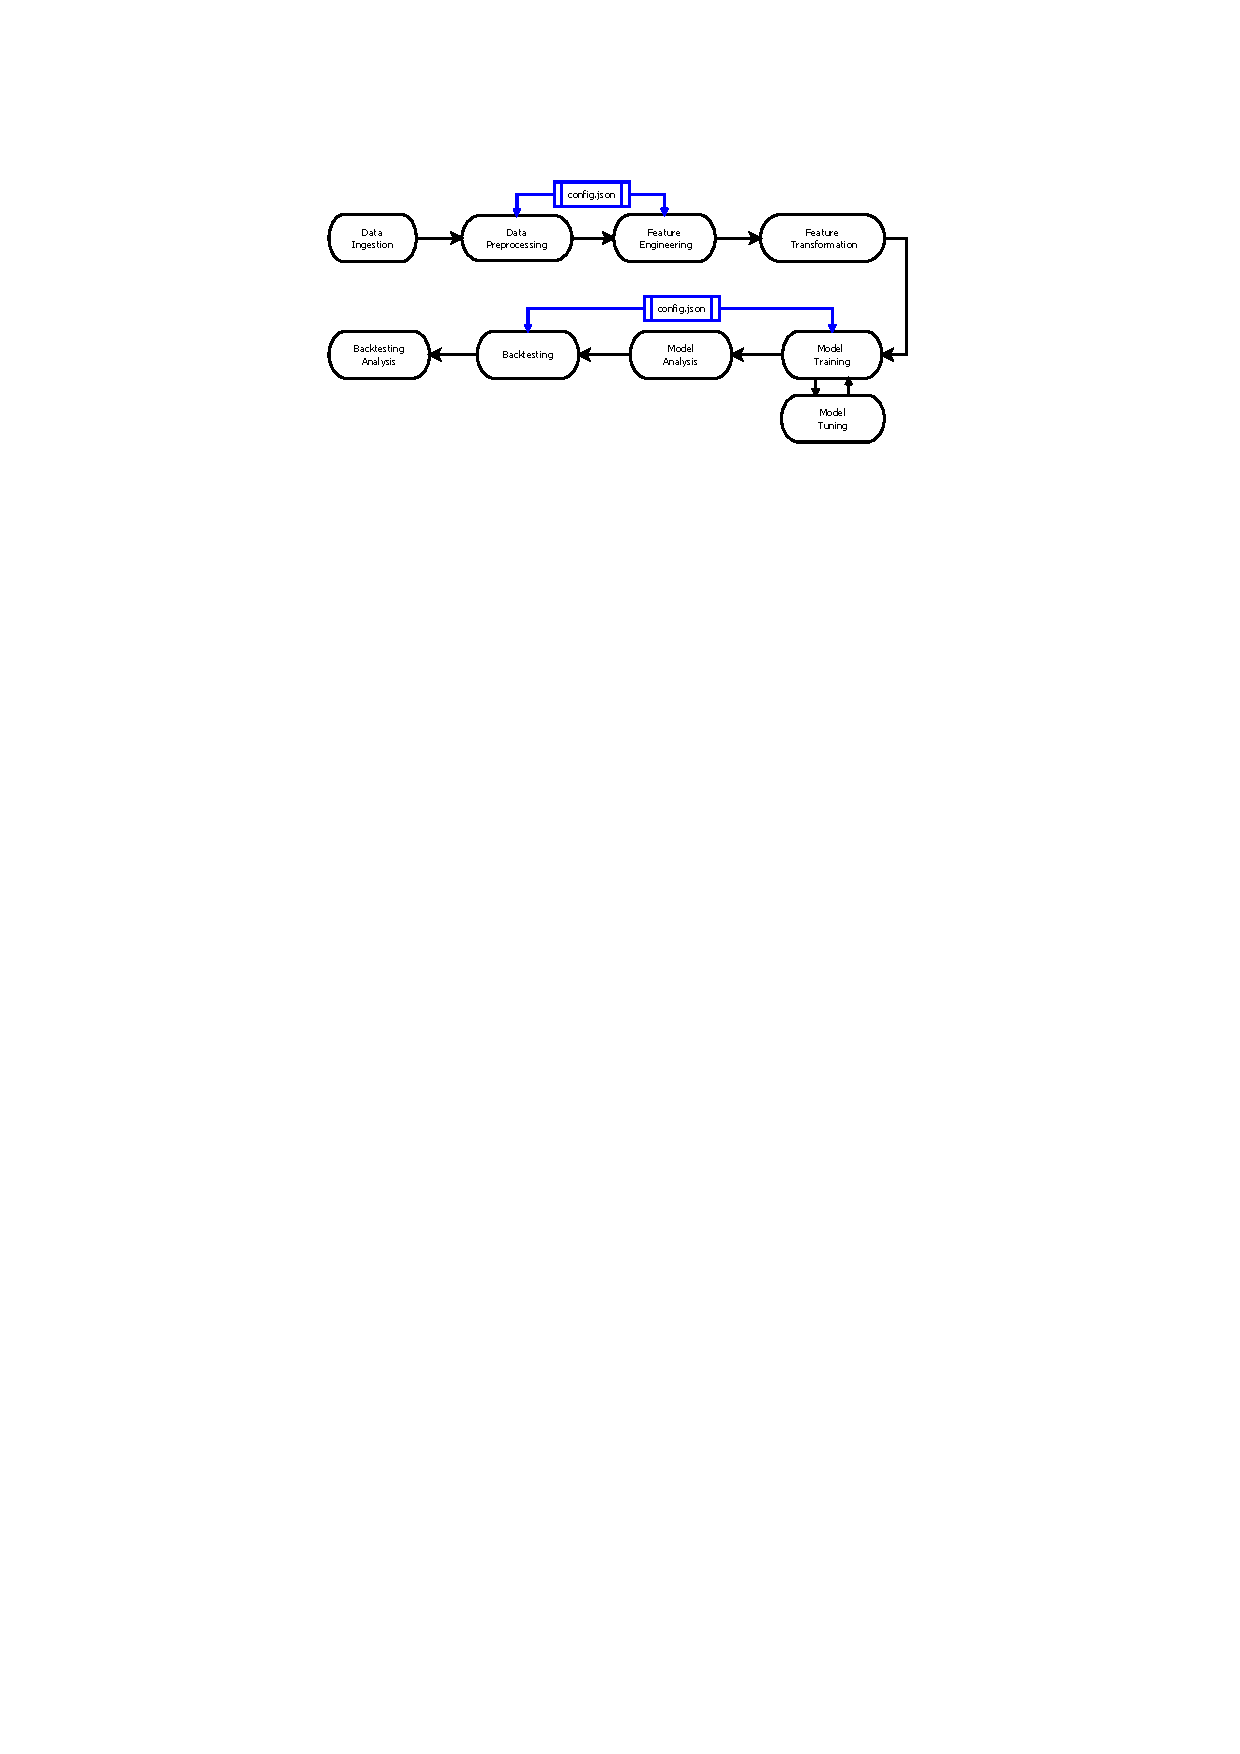
\includegraphics[trim=25mm 220mm 55mm 30mm, width=1.2\textwidth, clip]{./pdf/ml_pipeline.pdf}
\caption{Machine Learning Trading Pipeline: A visualization of the process, detailing steps from data acquisition and preprocessing, feature engineering and transformation, model training and optimizing, to the final execution and evaluation of trades based on model predictions.}
\label{fig:ml_pipeline}
\end{figure}

This pipeline initiates with raw historical data sourced from Binance and advances through a series of steps
leading to informed trading decisions. The process involves backtesting using the trained and optimized ML model on the historical data.
The pipeline steps can also be executed independently.
For instance, starting with data ingestion and preprocessing can be followed by feature engineering and data visualization to gain a deeper understanding of the dataset. The steps of the pipeline in  fig. \ref{fig:ml_pipeline}. are detailed in the subsequent subsections.

\subsection{ML Trading Pipeline Configuration}
The following JSON configuration in lst. \ref{lst:pipeline_conf} is used to set up the machine learning pipeline.
The \texttt{dataset\_conf} element specifies details such as the cryptocurrency symbol to be backtested (BTCUSDT in this case), the frequency of the time series data, and the start and end dates. Additionally, it offers an option to set the date for splitting the dataset into training and test sets.
The configuration also includes options to set the desired model and specify the parameter ranges. This enables fine-tuning via grid search for the selection of optimal parameters.
Also the \texttt{target\_conf} element allows for the selection of the target for the classification model. There are several target variants to choose from, that are describe later.




\begin{lstlisting}[style=jsonstyle, caption={Machine Learning Pipeline Configuration},  captionpos=b, label=lst:pipeline_conf][h]
{
  "tc": 0.001,
  "dataset_conf": {
     "symbol": "BTCUSDT",
     "freq": "1d",
     "start_date": "2018-01-01 00:00:00",
     "end_date": "2023-08-30 23:59:00",
     "split_date": "2022-12-31 23:59:00",
     "mode": "full",
     "target_conf": {
       "target": "Exceed_Avg_Returns"
    }
  },
  "model_name": "RandomForestClassifier",
  "model_type": "classification",
  "models_config": [
     {
       "model": "AdaBoostClassifier",
       "params": {
          "n_estimators": [10, 30, 100],
          "learning_rate": [0.01, 0.1, 1.0],
          "algorithm": ["SAMME", "SAMME.R"]
       }
     }
  ]
}
\end{lstlisting}



\subsection{Data Ingestion and Preprocessing}
The first step involves ingesting the data required for backtesting. This data can be sourced from Binance using the \texttt{data\_retrieve.py} module, as detailed in the previous chapter.
The data is saved in the \texttt{historical\_data} folder, which is located within the corresponding symbol's subfolder, created during the data download process.
Once the data has been retrieved, it can be ingested into the pipeline. It's recommended to retrieve data with a one-minute time bar length,
as this can be efficiently downsampled later for larger intervals such as an hour or a day.
This is done during the data preprocessing phase. The ingested data is downsampled based on the bar length specified in the configuration (refer to \lstinline[label=lst:pipeline_conf]{lst:pipeline_conf}, line 5), where the \texttt{freq} parameter is set to \texttt{1d}.
Furthermore, a validation check is run to ensure data integrity.

%\vspace{20mm} % Put space between figure and subsection title
%\vspace{10mm} % Adjust the value to your liking
\FloatBarrier % This ensures that the figure is placed before continuing with the subsequent content
\subsection{Feature Engineering}
Feature engineering is a critical step in improving the model's predictive capability.
The goal is to identify features that could potentially influence the model's performance.
Technical indicators are utilized to create features that help models predict upcoming price movements based on historical market data.
The technical indicators used in the \texttt{ml\_feature\_engineer} module can be broadly categorized into momentum-based, trend-based, and volume-based.


\begin{itemize}
    \item \textbf{Momentum-based Indicators:} These are primarily concerned with the speed of price movements. Features like Rate of Change (ROC), Momentum, variations of the Stochastic Oscillator, and the Relative Strength Index (RSI) fall into this category.

    \item \textbf{Trend-based Indicators:} Aimed at identifying the movement direction over time, these include indicators such as the Moving Average (MA) and the Exponential Moving Average (EMA).

    \item \textbf{Volume-based Indicators:} Volume, in trading, refers to the number of shares or contracts traded in a security or market. The feature set for this category includes the On-Balance Volume (OBV).
\end{itemize}

\begin{lstlisting}[style=pythonstyle, language=Python, caption={Function to add features to the dataset},  captionpos=b, label=lst:add_features_function]
def add_features(self):
    """Add various technical indicators to the dataset."""
    for n in self.periods:
        self._add_ma(n)
        self._add_ema(n)
        self._add_rsi(n)
        self._add_sto(n)
        self._add_mom(n)
        self._add_roc(n)
        self._add_stos(n)
        self._add_stomom(n)
        self._add_storoc(n)
        self._add_stoch_rsi(n)
        self._add_sto_cross(n)
    self._add_obv()
    self._add_returns()
    self._add_rolling_cum_returns()
    self._add_rolling_cum_range()
    self._add_day_of_week()
    self._calculate_range()

\end{lstlisting}


Following this, a target is computed, which can also be specified in the configuration file. The available target variants include:
\begin{itemize}
    \item \textbf{Simple}: Predicts if the next day's price will go up or down based on today's closing price.
    \item \textbf{MA\_Relative}: Checks if today's closing price is above its short-term average and rising.
    \item \textbf{Momentum}: Examines if the stock's momentum is positive and increasing.
    \item \textbf{ROC}: Looks at if the rate of change (ROC) is positive and on the rise.
    \item \textbf{Consecutive\_Increases}: Predicts if returns will rise for the third consecutive time after a decline.
\end{itemize}

\begin{figure}[h]
\centering
\begin{adjustbox}{max width=1\textwidth,center}
    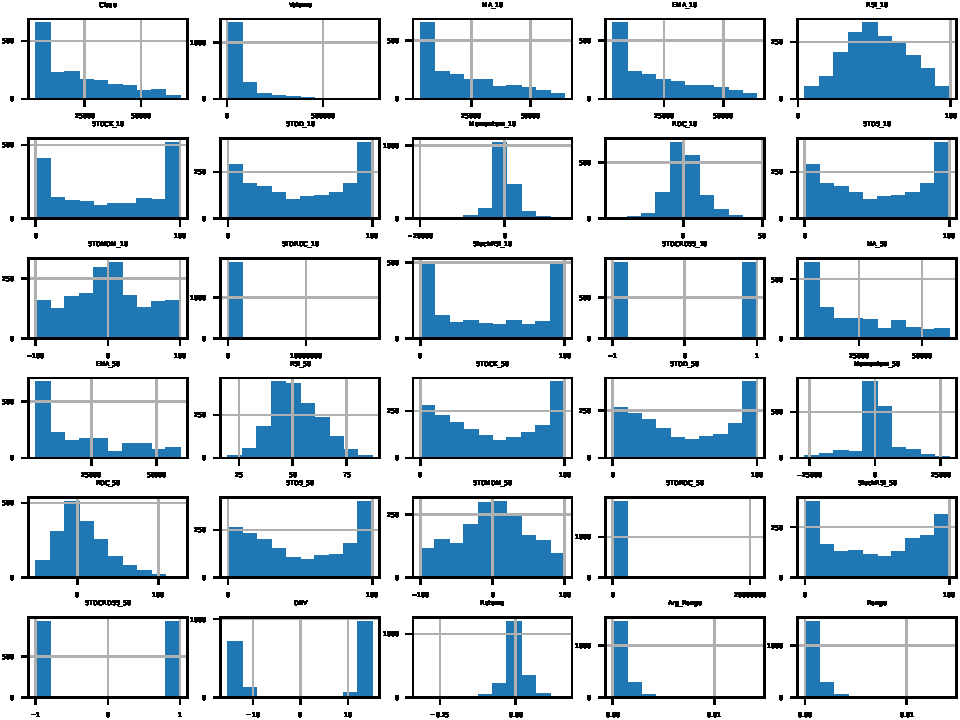
\includegraphics[scale=1]{./pdf/dataset_histogram.pdf}
\end{adjustbox}
\caption{Histogram of engineered features from the BTCUSDT historical data.}
\label{fig:dataset_histogram}
\end{figure}

 %Confusion matrix (left) presenting actual versus predicted values, alongside key performance metrics (right) indicating the model's accuracy, precision, recall, and F1 score.}
\subsection{Feature Transformation}

After engineering the features, it's essential to transform them to meet the specific requirements of machine learning models. Many algorithms have assumptions about the data's scale and distribution.
Hence, features undergo transformations using techniques like \texttt{Standardization} and {MinMax Scaling}.

It's importan to apply the same transformations with according parameters, to both the training and testing datasets or any new incoming data. This ensures consistent and accurate model predictions.

The entire transformation workflow, from data loading, preprocessing, to feature-related operations, is orchestrated by the \texttt{DataManager} and \texttt{FeatureEngineer} classes (fig. \ref{fig:dataManagerFeatureEngineer}).



\subsection{Data Visualization}
For data analysis the \texttt{ml\_model\_evaluator} module was implemented with appropriate methods. It provides tools for both data and model checks.
The prepared data can be visualized in various ways, including target distributions, feature covariance matrices, and feature histograms.

The \textbf{distribution of the predicted variable} across both training and validation datasets is showed in fig. \ref{fig:signal_distribution}.
Notably, the distribution between the two classes (1's and 0's) is nearly balanced in both datasets. Such a balanced distribution is crucial for training machine learning models effectively, ensuring that they aren't biased towards one class.

\begin{figure}[h]
\centering
\begin{adjustbox}{max width=1\textwidth,center}
    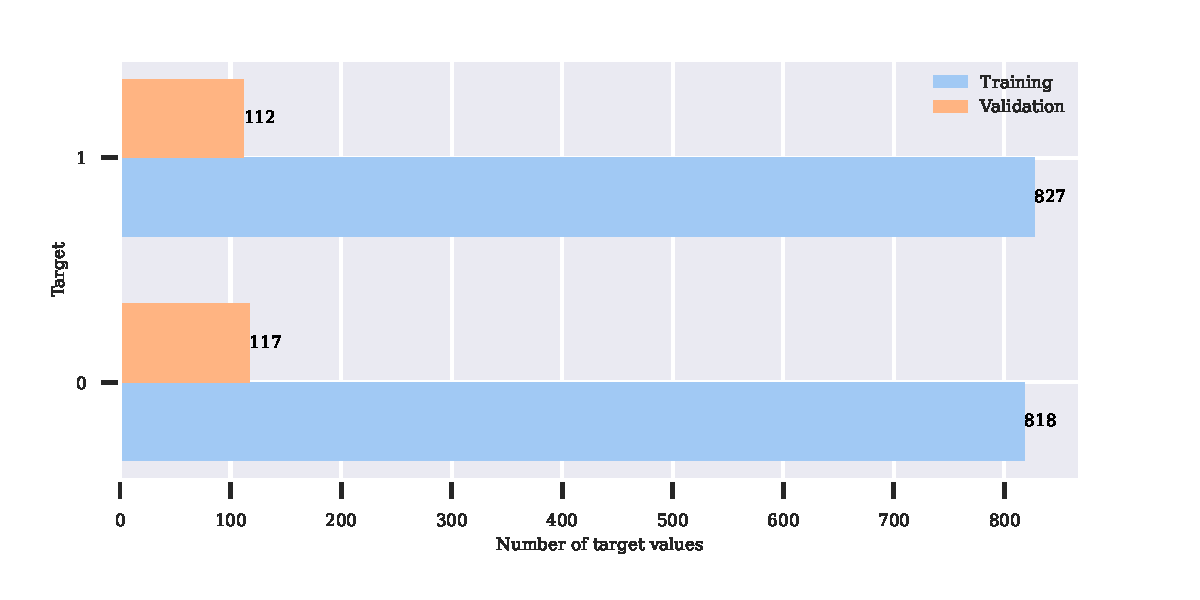
\includegraphics[scale=1]{./pdf/report/sig_distr.pdf}
\end{adjustbox}
    \caption{The distribution of target values in both the training testing datasets.}
\label{fig:signal_distribution}
\end{figure}

The fig. \ref{fig:corr_coef} illustrates the \textbf{correlation coefficients} between various feature variables in the dataset.
Each cell in the matrix represents the degree of correlation between two features: a value close to 1, represented by dark green, signifies a strong positive correlation, while a value close to -1, shown in white, indicates a strong negative correlation.

%trim=left bottom right top,
\begin{figure}[h]
\centering
\begin{adjustbox}{max width=1.2\textwidth,center}
    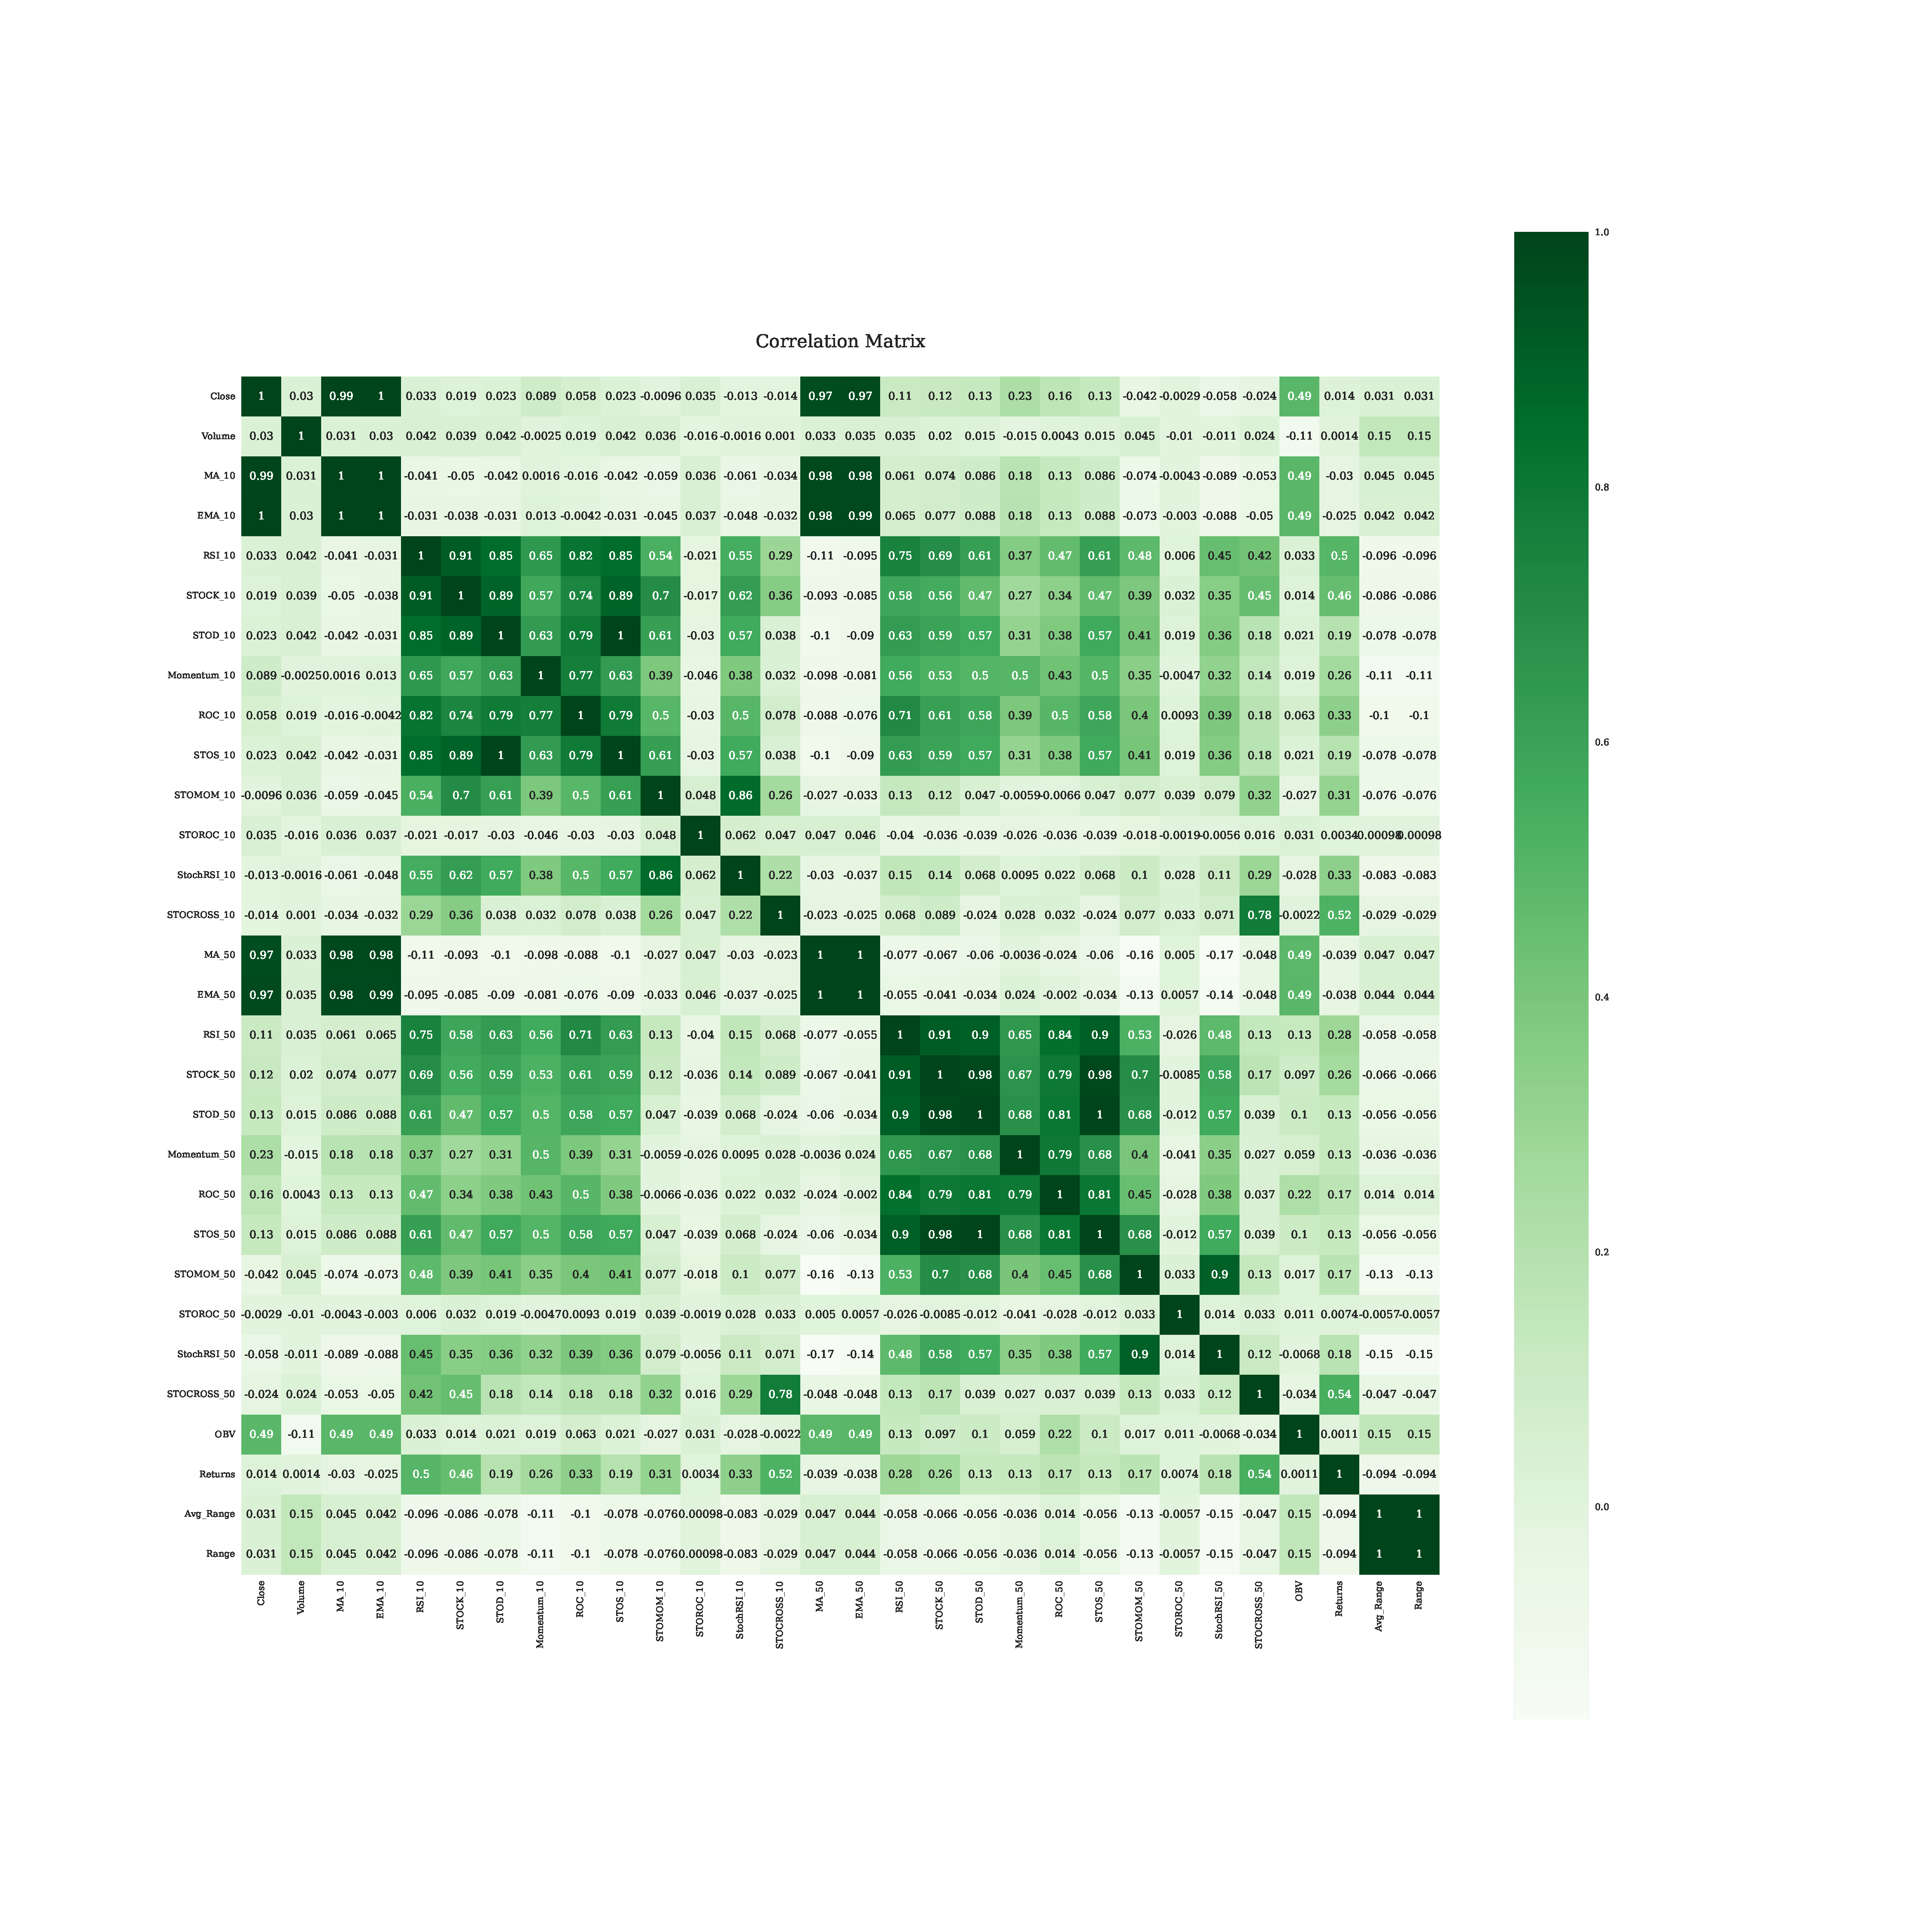
\includegraphics[scale=1.2, trim={30mm 70mm 50mm 110mm}, clip]{./pdf/correlation_matrix.pdf}
\end{adjustbox}
\caption{Correlation Coefficient between features variables.}
\label{fig:corr_coef}
\end{figure}

The fig. \ref{fig:dataset_histogram} presents a \textbf{histogram} showcasing the distribution of engineered features derived from the BTCUSDT historical data. Each bar in the histogram represents the frequency of occurrences for a particular value or range of values. This visualization provides insights into the distribution patterns and potential skewness of the different features in the dataset.



\subsection{Model Training and Optimization}
The logic for model training and backtesting is encapsulated within the \texttt{ml\_backtester.py} module,
while the \texttt{ml\_optimizer.py} module is dedicated to optimization purposes, as depicted in Figure \ref{fig:<your_figure_label_here>}.
The \texttt{\_optimize\_model} function in the \texttt{ml\_backtester.py} module is responsible for the model optimization process.
It utilizes the instance of the MlOptimizer class to perform searching for the best parameters of the model using techniques such as Grid Search with Cross-Validation.
In a grid search, a grid of all possible hyperparameter combinations is created, and the model is trained using each one of them. The best model is then used in the \texttt{\_generate\_predictions}
function to predict the trends in price movements on unseen data. Once optimized, the trained model specific to a cryptocurrency can be saved for subsequent use and reloaded as needed.
Model specifics, such as the model type (for instance, AdaBoostClassifier) and its hyperparameter ranges, are defined in the JSON configuration file (see lst. \ref{lst:pipeline_conf}).

\begin{lstlisting}[style=pythonstyle, language=Python, caption={Function of MlBacktester class for model optimization and predictions.},  captionpos=b, label=lst:add_features_function]
def _optimize_model(self):
   # Instantiate the GridSearchOptimizer
   optimizer = GridSearchOptimizer(self.data_manager.X_train,
                                self.data_manager.y_train,
                                self.config.dataset_conf.symbol,
                                task_type=self.config.model_type,
                                num_folds=self.config.num_folds,
                                scoring=self.config.scoring)

   # Optimize the model using configured parameters grid
   best_model = optimizer.grid_search(self.config.model_name,
                                  self.model,
                                  self.get_model_params_grid())

   # Update the model of the strategy to the optimized model
   self.model = best_model

def _generate_predictions(self):
   '''Generate predictions using the model.'''
   predictions = self.model.predict(self.data.X_train)
   self.data['predictions'] = predictions
   self.data['predictions'].ffill().fillna(0, inplace=True)

\end{lstlisting}

\subsection{Model Evaluation using Classification Metrics}
After training the trading model's performance can be evaluated using several metrics. These metrics provide insights into the model's predictions and highlight potential areas for improvement.
The performance data for both the training and testing of the model are visualized in fig. \ref{fig:conf_matrix}.
For each phase (training and testing):

The left diagram presents the confusion matrix, which shows the number of correct and incorrect predictions made by the model.
The right diagram visualizes key performance metrics, specifically: accuracy, precision, recall, and F1 score. Each metric is also further described in  more detail below.
\begin{figure}[h]
    \centering

    \begin{subfigure}[b]{\textwidth}
        \begin{adjustbox}{max width=0.8\textwidth,center}
            \includegraphics[scale=0.8]{./pdf/report/report\_train.pdf}
        \end{adjustbox}
        \caption{Model Performance Metrics based on Training Data.}
        \label{fig:train_perf}
    \end{subfigure}

    \bigskip % Adds some vertical space between the two subfigures

    \begin{subfigure}[b]{\textwidth}
        \begin{adjustbox}{max width=0.8\textwidth,center}
            \includegraphics[scale=0.8]{./pdf/report/report\_test.pdf}
        \end{adjustbox}
        \caption{Model Performance Metrics based on Testing Data.}
        \label{fig:test_perf}
    \end{subfigure}

    \caption{Visualization of the Classification Report.}
    \label{fig:conf_matrix}
\end{figure}

\begin{itemize}
	\item \textbf{True Positive:} Represents the number of times the model correctly predicted an upward trend and the price actually went up.

	\item \textbf{True Negative:} Represents the number of times the model correctly predicted a downward trend and the price actually went down.

	\item \textbf{False Positive:} Represents the number of times the model incorrectly predicted an upward trend and the price went down or stayed the same. This type of error could result in a missed shorting opportunity or a loss if one decided to buy in Long Only strategies.

	\item \textbf{False Negative:} Represents the number of times the model incorrectly predicted the downward trend and the price went up or stayed the same. This type of error could result in missed profit opportunities from not buying.

	\item \textbf{Recall:} The ratio of the number of correct positive predictions (TP) to the total actual positives (TP + FN). In mathematical terms, Recall $= \frac{TP}{TP + FN}$. In trading, it indicates how well the model identifies actual upward movements. A high recall means the model captures most of the upward trends, but this can also be achieved at the expense of more false positives.

	\item \textbf{Precision:} The ratio of correct positive predictions (TP) to the total predicted positives (TP + FP). In mathematical terms, Precision $= \frac{TP}{TP + FP}$. Shows how many of the predicted upward trends by the model were actually correct. High precision means that when the model predicts an upward trend, it's likely correct. But a higher precision might come at the expense of missing some actual upward trends (lower recall).

	\item \textbf{Accuracy:} The ratio of correct predictions (both TP and TN) to the total number of predictions (TP + TN + FP + FN). In mathematical terms, Accuracy $= \frac{TP + TN}{TP + TN + FP + FN}$. In trading, it gives an overall measure of how often the model is correct, regardless of whether it's predicting upward or downward movement.

	\item \textbf{F1 Score:} The harmonic mean of precision and recall, providing a balance between the two. It is given by the formula: F1 $= 2 \times \frac{\text{Precision} \times \text{Recall}}{\text{Precision} + \text{Recall}}$. It's especially useful when the class distribution is imbalanced. In trading, a high F1 score suggests the model has a balanced performance in terms of identifying upward trends and avoiding false alarms.
\end{itemize}


\subsection{Backtesting and Analysis}
After the model is trained and fine-tuned, it's crucial to check how good it is by testing its effectiveness not just on the basis of typical classification metrics but also on how well it performs in a simulated trading environment.

The code listing \ref{lst:add_features_function} showcases the \texttt{run\_strategy} function, a part of the \texttt{MlBacktester} class. This function is designed to run the backtesting process:

\begin{figure}[h]
\centering
\begin{adjustbox}{max width=1.3\textwidth,center}
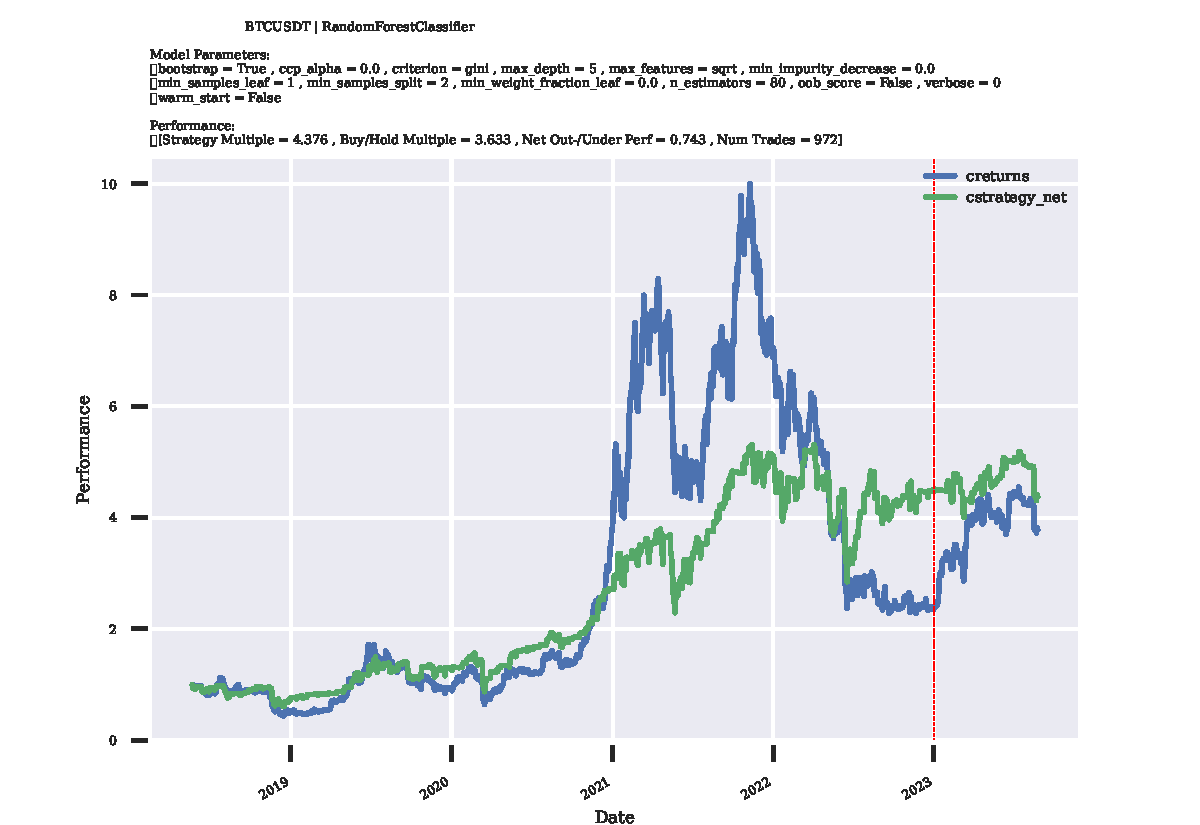
\includegraphics[scale=1.3]{./pdf/report/backtest_res.pdf}
\end{adjustbox}
\caption{Feature Significance in Model Prediction}
\label{fig:backtest_res}
\end{figure}

After generating predictions, the strategy values are calculated. These strategy values reflect the positions the model would take based on its predictions.
Further, trades are determined and adjustments are made to account for transaction costs, which are often overlooked but can significantly impact net returns in real-world scenarios.
Finally, cumulative metrics are computed, followed by a performance evaluation to assess the overall success of the trading strategy.
By summing the strategy returns, the model's hypothetical profitability over the backtesting period is determined.

\begin{lstlisting}[style=pythonstyle, language=Python, caption={\vspace*{1cm}Function of MlBacktester class for backtesting execution.},  captionpos=b, label=lst:add_features_function]
def run_strategy(self):
    '''Backtests the trading strategy.'''
    self._generate_predictions()
    self._calculate_strategy_values()
    self._calculate_trades()
    self._adjust_for_transaction_costs()
    self._calculate_cumulative_metrics()
    self.perf_evaluator._calculate_perf(self.data)

\end{lstlisting}

A common benchmark to assess the strategy's success is the "buy and hold" method.
In this approach, the asset is bought and kept throughout the entire period without incurring extra costs or decisions based on price changes.
Comparing the total strategy returns to the "buy and hold" method's returns provides an understanding of the ML-based strategy's added benefit.
If the model outperformes this benchmark, it can be considered as useful for trading.

The fig. \ref{fig:backtest_res} illustrates the comparison between the returns of the "buy and hold" strategy and those of the configured \texttt{AdaBoostClassifier} model's strategy.
The model's strategy achieved a return multiple of 4.376. This surpasses the 3.633 return from the "buy and hold" method, resulting in a net outperformance of 0.743, or 74.3\%.
This outperformance is observed at the end of the backtesting period, which can also be configured in the JSON configuration shown in lst. \ref{lst:pipeline_conf}.
Moreover, the analysis took into account Binance's trading fees of 0.1\% for spot trading, ensuring a more realistic representation of potential real-world returns.
The backtesting results show the potential of the model for real-world trading scenarios.





\begin{figure}
\centering
\begin{adjustbox}{max width=1.2\textwidth,center}
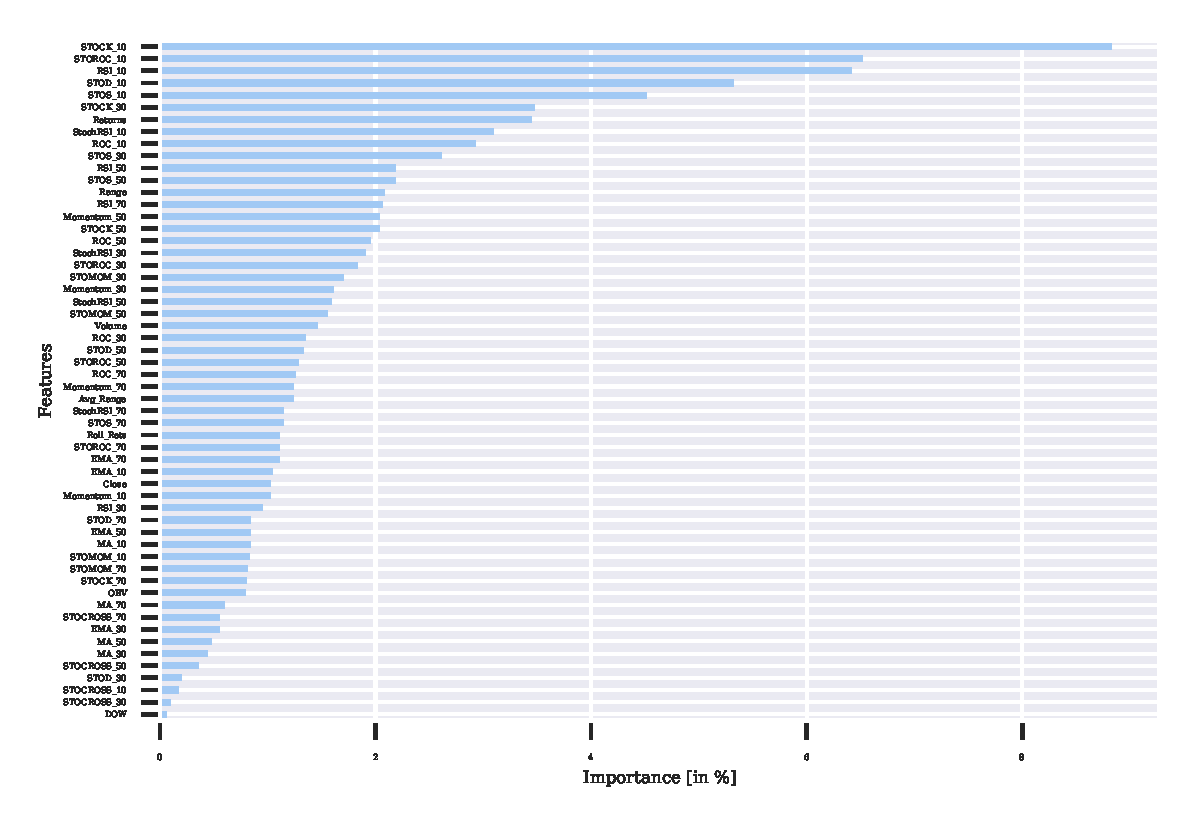
\includegraphics[scale=1.2]{./pdf/report/feature_importance.pdf}
\end{adjustbox}
\caption{Feature Significance in Model Prediction}
\label{fig:feature_importance}
\end{figure}


\begin{figure}[h]
\centering
\includegraphics[width=0.9\textwidth]{./pdf/report/explained\_variance.pdf}
\caption{Explained Variance of Features after Performing Feature Reduction.}
\label{fig:explained_variance}
\end{figure}
